\section{Architectural state and access to history}
\label{sec:C03:architectures}
The Transformer makes a position-dependent representation by mixing previous token representations through attention and applying learned nonlinear transformations. For one attention head, $Q=XW_Q$, $K=XW_K$, and $V=XW_V$, with $\operatorname{softmax}(QK^\top/\sqrt{d_h}+A)V$ defining the output under additive mask $A$. A causal mask prevents access to future positions. This is a constraint on the computational graph, not a claim that the representation is a faithful account of everything in the past. Positional information, finite precision, training distribution, and learned attention patterns all affect what historical evidence influences a decision~\cite{vaswani2017attention}.

Dense attention offers direct content-dependent access to retained positions, with quadratic attention arithmetic during a full sequence pass. A recurrent architecture compresses past information into a bounded state. Transformer-XL introduces segment-level recurrence, while selective state-space models such as Mamba use input-dependent state updates designed for efficient sequence processing~\cite{dai2019transformerxl,gu2023mamba}. The important comparison for agents is not whether an architecture has memory in an informal sense. It is what can be retained, accessed, modified, or invalidated under a fixed storage and computation envelope. A recurrent state can be compact while losing a rare constraint that an external event log still preserves.

Consider a deterministic recurrent update $z_{t+1}=f_\theta(z_t,x_t)$. If two distinct histories map to the same $z_t$, every subsequent decision based only on that state must treat them identically until new observations distinguish them. When the histories require different authorized actions, this state aliasing imposes an irreducible error for that interface. Attention can avoid that particular collision by retaining explicit positions, but it does not eliminate errors of selection or interpretation. External retrieval changes the accessible evidence again. Consequently, a fair comparison must hold the external memory service constant or explicitly attribute gains to the combined architecture.

Rotary position embeddings encode relative phase relationships in queries and keys. Their algebraic ability to evaluate larger positions does not establish useful reasoning at those positions~\cite{su2021roformer}. Extending a context window can change frequency regimes, attention distributions, and numerical behavior. An agent with a long session also encounters a nonuniform evidence distribution: recent tool responses, early user constraints, and intermediate summaries have different roles. Tests that merely insert one recoverable string into a long input do not fully measure the ability to reconcile those roles. Nominal length and effective decision context therefore require separate reporting.

Mixture-of-experts architectures introduce conditional parameter activation. A router selects a small subset of experts for each token, so total stored parameters exceed the parameters active in one forward path~\cite{shazeer2017moe}. This can improve the capacity-to-compute tradeoff, but expert weights still occupy memory and communication can dominate when routing crosses devices. An agent workload with small batches and heterogeneous contexts may exercise a different routing and communication regime from the large packed sequences used in training. Total parameter count is thus insufficient to predict latency, cost, or quality. Active FLOPs, resident memory, expert imbalance, and interconnect behavior belong in the comparison.

Grouped-query attention shares key and value heads across groups of query heads. It reduces the dimensionality of cached keys and values while retaining multiple query projections~\cite{ainslie2023gqa}. The reduction in KV storage is exact for a specified layout; the quality effect is empirical and depends on training or conversion. Calling grouped-query attention a larger context mechanism is incomplete: it makes a given capacity cheaper, but does not guarantee that the model uses additional historical information correctly. The distinction matters when a product increases the advertised window after an infrastructure change without changing its evidence-use evaluation.

Multi-head latent attention uses a different factorization. The DeepSeek-V3 report's Section 2.1.1 jointly compresses content keys and values into a latent vector and retains a separate rotary-position component~\cite{rewrite_deepseek3mla}. In schematic column-vector notation, let $c_j=W_Dh_j$, $k_j^C=W_Kc_j$, and $v_j=W_Vc_j$. The content score obeys $q_i^\top W_Kc_j=(W_K^\top q_i)^\top c_j$, allowing a compatible implementation to score against the compressed state without storing every expanded content key. The separate positional contribution must still be handled; ignoring it does not reproduce the trained attention computation.

If the retained latent has dimension $r$ and the extra positional key has dimension $d_R$, an ideal per-token cache stores $r+d_R$ elements instead of $2hd_h$ for ordinary equal-width multi-head keys and values. This is a shape-based accounting identity, not a quality guarantee or an assertion that every implementation achieves the ideal storage. Up-projection arithmetic, query transformations, tensor layout, and kernel support affect performance. For an agent, this architecture changes the cost of preserving a long interaction history while leaving the separate question of decision-relevant recall unresolved. It should be compared with grouped-query and sparse-attention alternatives under matched quality and actual serving workloads.

\subsection{Shared computational state in looped Transformers}
\label{sec:C03:looped}
The October 2026 Looped Prediction Transformer study trains repeated applications of a shared block stack to read the first recursion's full cache while retaining short local caches in later recursions. Its Section 3 specifies joint attention to shared and local entries in one softmax~\cite{rewrite_looped2026}. This is architectural recurrence within token prediction. It is neither a store of user sessions nor an ordinary deeper network with independently parameterized layers. The same parameters participate repeatedly, changing the computation and gradient paths without multiplying the stored block weights.

Let $L$ be the shared stack depth, $R$ its recursion count, $T$ the retained token count, and $w$ the local window for later recursions. Suppressing constant bytes and head dimensions, the two cache layouts have sizes
\begin{align}
 M_{\rm separate}&\propto LRT,\\
 M_{\rm shared}&\propto L[T+(R-1)w].
\end{align}
Their ratio is $[1+(R-1)w/T]/R$. At $R=5$, $T=4096$, and $w=64$, it is 0.2125. This calculated storage ratio does not imply a comparable reduction in computation: every recursion still evaluates the shared stack, and later queries read both shared and local evidence. Under the same simplified per-token read model, the extra local attention entries are a fraction $(R-1)w/(RT)=0.0125$ of the separate-cache baseline.

Parameter sharing also constrains the function class. Repeating one transformation does not reproduce an arbitrary sequence of independently trained transformations, while explicit shared-cache access changes the available state at each recursion. A useful experiment separates weight tying, recursion count, local-window size, and shared-cache visibility at matched training exposure. Detaching the shared-cache gradient path tests a different mechanism from merely preventing later recursions from reading it. The source study analyzes these distinctions, but no universal benefit of increasing recursion depth follows from the architecture alone.

For agents, internal recursion spends computation without acquiring a new external observation. It can refine a prediction from existing evidence, but cannot resolve an unobserved transaction outcome by itself. Its cache remains tied to the model computation and does not establish durable cross-session memory. Compare extra internal recursions with external sampling, tool verification, or another observation under a declared cost envelope. These alternatives supply different information, so both their resource use and their evidence access must be reported when attributing gains to deeper reasoning.



The projection placement changes which quantities require expansion (Figure~\ref{fig:C03:latent-score}).
\begin{figure}[!htbp]
\centering
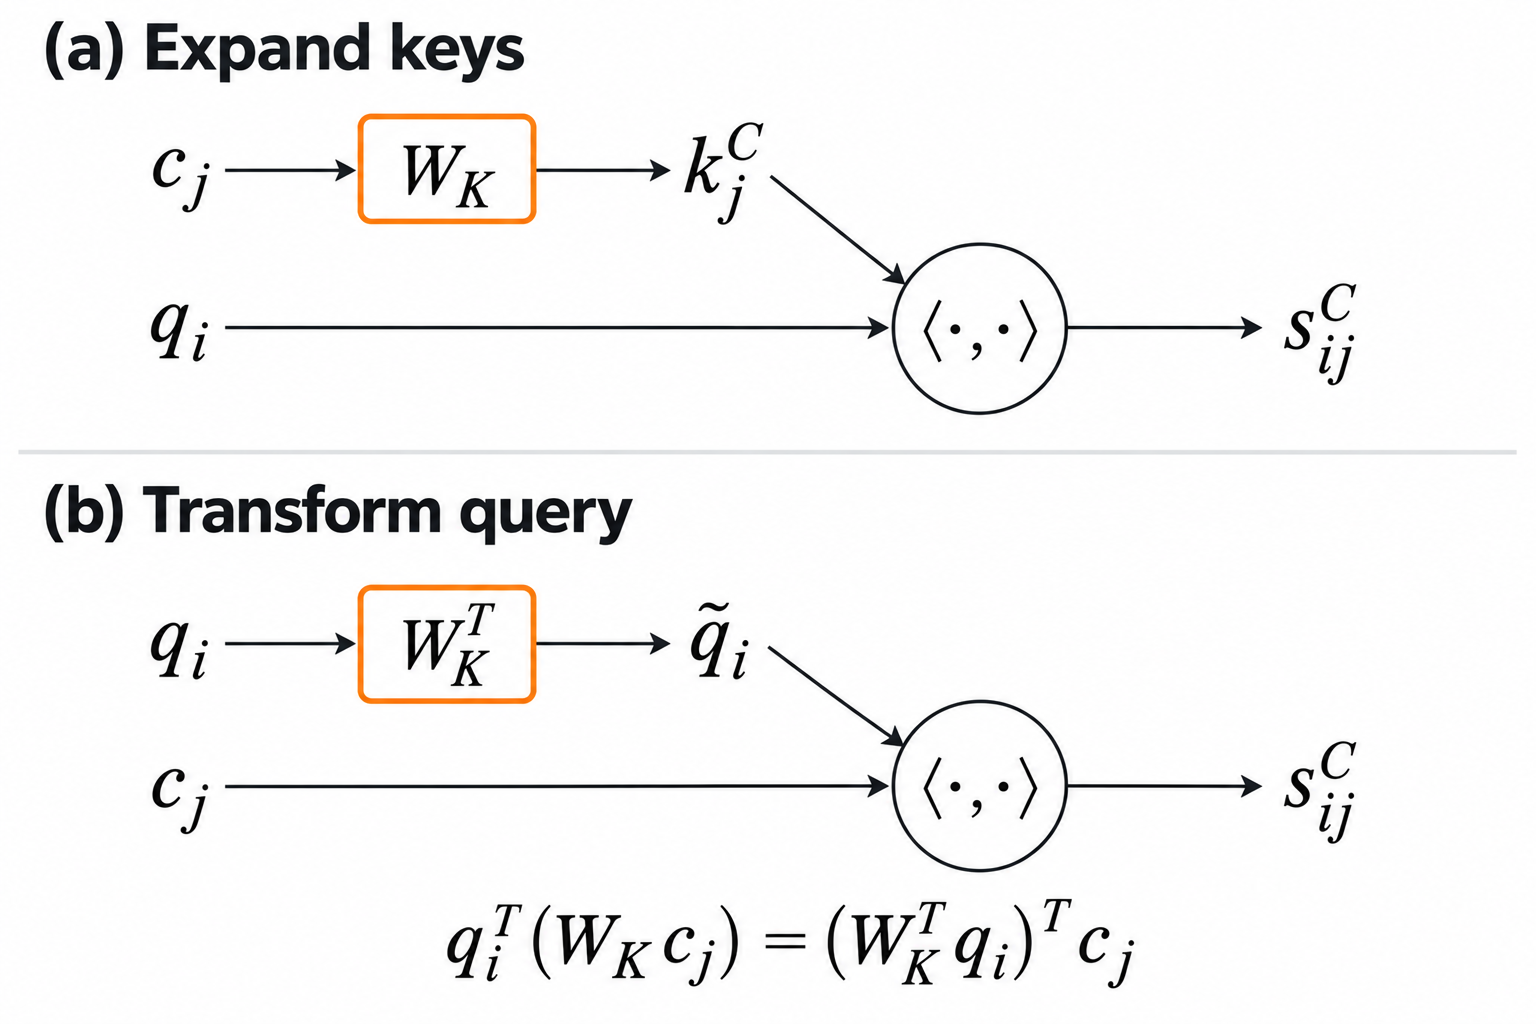
\includegraphics[width=\linewidth]{book/figures/assets/F03review.png}
\caption{Two algebraically equivalent content-score paths, $s_{ij}^C=q_i^\top(W_Kc_j)=(W_K^\top q_i)^\top c_j$, with transformed query $\widetilde q_i=W_K^\top q_i$. Moving the linear projection permits a compatible implementation to score retained latents without storing expanded content keys. The positional score and value path are omitted; finite-precision implementations require numerical comparison. No measured performance result is depicted.}
\label{fig:C03:latent-score}
\end{figure}
